
\documentclass[10pt,twocolumn,letterpaper]{article}
\usepackage{array}
\usepackage{statcourse}
\usepackage{times}
\usepackage{epsfig}
\usepackage{graphicx}
\usepackage{amsmath}
\usepackage{amssymb}
\usepackage{booktabs}
\usepackage{multirow}
\usepackage{caption}

% Include other packages here, before hyperref.

% If you comment hyperref and then uncomment it, you should delete
% egpaper.aux before re-running latex.  (Or just hit 'q' on the first latex
% run, let it finish, and you should be clear).
\definecolor{cvprblue}{rgb}{0.21,0.49,0.74}
\usepackage[breaklinks=true,bookmarks=false,colorlinks,citecolor=cvprblue]{hyperref}

\statcoursefinalcopy%

\setcounter{page}{1}
\begin{document}


%%%%%%%%%%%%%%%%%%%%%%%%%%%%%%%%%%%%%%%%%%%%%%%%%%%%%%%%%%%%%%%
% DO NOT EDIT ANYTHING ABOVE THIS LINE
% EXCEPT IF YOU LIKE TO USE ADDITIONAL PACKAGES
%%%%%%%%%%%%%%%%%%%%%%%%%%%%%%%%%%%%%%%%%%%%%%%%%%%%%%%%%%%%%%%



%%%%%%%%% TITLE
\title{Comparative Analysis of Machine Learning Models: \\Alexnet, VGG, ResNet, YOLO}

\author{Pham Duc An\\
{\tt\small 10422002}
\and
Tran Hai Duong\\
{\tt\small 10422021}
\and
Vo Thi Hong Ha\\
{\tt\small 10421015}
\and
Nguyen Hoang Anh Khoa\\
{\tt\small 10422037}
\and
Truong Hao Nhien\\
{\tt\small 10422062}
\and
Nguyen Song Thien Phuc\\
{\tt\small 10422067}\\
\\
Vietnamese-German University\\
\{\tt\small @student.vgu.edu.vn\}
\and
Bui Duc Xuan\\
{\tt\small 10422085}
}

\maketitle
%\thispagestyle{empty}



% MAIN ARTICLE GOES BELOW
%%%%%%%%%%%%%%%%%%%%%%%%%%%%%%%%%%%%%%%%%%%%%%%%%%%%%%%%%%%%%%%


%%%%%%%%% ABSTRACT
\begin{abstract}
    In this project, we conducted a comprehensive comparative analysis of prominent machine learning models, namely Alexnet, VGG, ResNet, and YOLO, with a focus on their efficacy in image recognition. Leveraging a curated dataset representative of diverse real-world scenarios with CIFAR-10, our study delved into the nuances of each model's architecture, training process, and computational requirements. Through rigorous evaluation using metrics such as accuracy, precision, and recall, our results reveal nuanced performance distinctions. Notably, ResNet demonstrated superior accuracy, VGG excelled in feature extraction, YOLO showcased real-time efficiency, and Alexnet exhibited a stable performance. These findings provide valuable insights for practitioners and researchers seeking to optimize model selection for specific applications, shedding light on the trade-offs between accuracy, computational cost, and real-time processing capabilities. Project's detailed code are provided at {\url{https://github.com/nhientruong04/LIA-introCS-proj}}.
    % \small\paragraph{Keywords} Alexnet, VGG, ResNet, YOLO, Image Recognition, Deep Learning, Convolutional Neural Networks, Computer Vision, CIFAR-10.
\end{abstract}

%%%%%%%%% BODY TEXT
\section{Introduction}

Human cognitive processes, mirroring the intricacies of an advanced supercomputer\cite{hassan2019computer}, rely on the nuanced interaction of neurons to perceive diverse stimuli such as digits, numbers, words, and images. This cognitive evolution spans from its early stages to the present era, with a notable milestone being the introduction of not only Generative AI but also other groundbreaking advancements in artificial intelligence.

In an era defined by the rapid advancement of artificial intelligence, the field of machine learning and deep learning stands as a beacon of innovation, transforming the way computers perceive and interact with their surroundings. This project delves into the intricate world of these cutting-edge technologies, specifically focusing on computer vision—a domain crucial for tasks ranging from image recognition to object detection. With the four chosen prominent models-Alexnet\cite{Alexnet}, VGG\cite{VGG}, ResNet\cite{ResNet}, and YOLO\cite{yolov5}, we are seeking to unravel the complexities and reveal the engine behind these widely recognized models.

The comprehensive AI taxonomy proposed by IBM outlines seven distinct types, with Generative AI representing the initial stride in the AI continuum. Within this evolving landscape, Convolutional Neural Networks (CNNs)\footnote{\url{https://arxiv.org/pdf/1511.08458.pdf}} have garnered particular attention and proven to be a pivotal model. CNNs stand out for their remarkable application in various domains, excelling in tasks such as image classification, object detection, and pattern recognition.

In the realm of machine learning (ML), CNNs have risen to prominence, offering a competitive edge over traditional regression and statistical models, particularly in tasks requiring image analysis. Their efficacy is underscored by their ability to automatically learn hierarchical features from data, making them well-suited for complex visual tasks.

This paradigm shift exemplifies the dynamic nature of AI, where models like CNNs, designed to emulate the human visual system, have become indispensable tools in addressing intricate challenges across diverse disciplines.

The rest of this paper is organized as follows:

\paragraph{Literature review} Before delving into the specific machine learning models, it is crucial to contextualize this study within the existing body of knowledge. The literature review section provides a comprehensive overview of relevant research, identifying key advancements, methodologies, and challenges in the field of image recognition and machine learning. By synthesizing existing literature, we aim to establish a foundation for understanding the evolution of these models and highlight gaps that our study seeks to address.

\paragraph{Models} The following section explores four machine learning models-Alexnet, VGGNet, ResNet, and YOLO\@. We delve into their architectures, training nuances, and some key highlight that makes each of the models different.

\paragraph{Insightful summarization} The insightful summarization section provides a comprehensive comparative analysis of the four models, highlighting their strengths and weaknesses. We also discuss the implications of our findings for practitioners and researchers.

\paragraph{Challenges} Despite the remarkable strides made in the development of machine learning models, challenges persist. In this section, we identify and discuss key challenges encountered in the deployment and optimization of these models, offering insights into areas that demand further attention.

\paragraph{Experiments} The experiment section outlines the experimental setup, including the dataset, evaluation metrics, and implementation details. We then present the results of our experiments, highlighting the nuances of each model's performance.

\paragraph{Teamwork} The teamwork section provides a brief overview of the team's collaboration process, highlighting the key challenges and lessons learned.

\paragraph{Conclusion} Summarizes findings, highlighting nuanced performance distinctions, and discusses implications for practitioners. Outlines potential avenues for future research.

%%%%%%%%% LITERATURE REVIEW
\section{Literature review}

Deep learning methodologies have been widely applied in the detection and classification of images, with a multitude of research focusing on improving their precision and effectiveness. Each research study is unique, considering factors such as the specific type of tasks, the deep learning methods used, the performance metrics applied, and the datasets chosen. These factors could potentially affect the applicability of the models to different datasets. By categorizing these studies based on the specific type of tasks and the deep learning method used, we can identify similarities and differences, which could provide valuable insights for our current research. A significant number of studies have utilized convolutional neural networks (CNN) for object classification. For example, Krizhevsky et al.\cite{Alexnet} demonstrated the power of deep convolutional neural networks with AlexNet, a CNN with 8 convolutional layers and shows that it achieves a top-1 error rate of 15.3\% on the ImageNet classification task. This success paved the way for the development of deeper CNNs such as VGG and ResNet. Simonyan et al.\cite{VGG} present a novel architecture for convolutional neural networks (CNNs) that enables the training of extremely deep networks (VGGNets)  and achieved state-of-the-art results,with a top-1 error rate of 5.1\% on the ImageNet classification task. Similarly, Zhang et al.\cite{ResNet} introduced the Deep Residual Learning (DRL) framework, which achieves record-breaking results  attaining a 3.57\% top-1 error rate for 152 layers on the ImageNet classification task. DRL introduces residual connections, which allow for the construction of much deeper networks without vanishing gradients. Despite these promising results, these CNNs models are limited in training and data related. Some studies employ other pipelines which include advanced techniques to get a better result in classification. Redmon et al.\cite{Yolo} used an unified framework algorithm, YOLO\@. With the assistance of the framework, it performs both object detection and classification in a single pass of the input image. YOLO is able to execute within a short period of time, while achieving comparable accuracy. These four models have been extensively studied and evaluated in the literature. For example, a comprehensive review of deep learning models for object detection by Vaswani et al. (2020)\cite{Review} compared the performance of AlexNet, VGG, ResNet, and YOLO on a variety of object detection datasets. The review found that ResNet and YOLO generally outperformed AlexNet and VGG on all datasets. These models have been shown to achieve state-of-the-art results on a variety of image recognition and object detection tasks. However, AlexNet, VGG, ResNet, and YOLO are still widely used in practice due to their simplicity, robustness, and accuracy.


%%%%%%%%% MODELS

\section{Models}
\subsection{AlexNet}
In 2012, the ImageNet Large Scale Visual Recognition Challenge (ILSVRC)\footnote{\url{https://image-net.org/challengehttps://image-net.org/challenges/LSVRC/index.phps/LSVRC/index.php}} dataset was introduced, which required a model capable of processing a large dataset like ImageNet. The introduction of Alexnet by Alex Krizhevsky, Ilya Sutskever, and Geoffrey E. Hinton marked a significant milestone in the field of computer vision. Alexnet showed the feasibility of deep learning so well that it got a top-five error of fifteen point three percent on data that has a thousand categories in the ILSVRC 2012\cite{Alexnet}. Its original paper is the theoretical basis for the report below.
\subsubsection{Overall architecture}

\begin{flushleft}
    \begin{figure}[h!]
        \begin{center}
            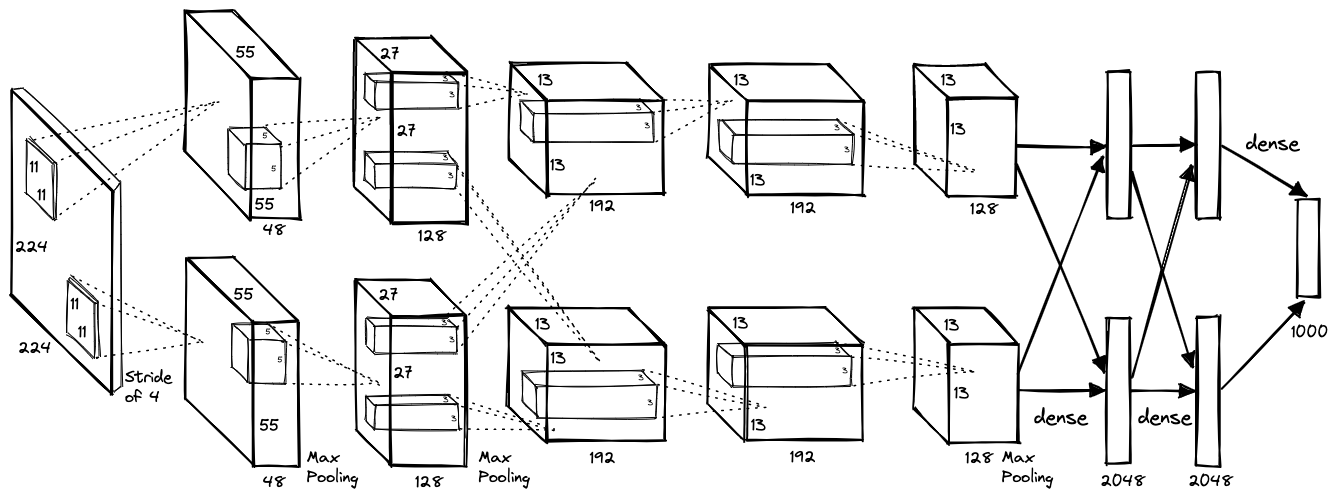
\includegraphics[scale=0.15]{figures/imagenet-6.png}
            \caption{An illustration of the architecture of AlexNet, clearly demonstrating the division of responsibility between the two GPUs.}\label{fig:imagenet-6}
        \end{center}
    \end{figure}
\end{flushleft}
% \footnotetext{The input size is mentioned at most of the places as 224*224*3 but due to some special reason which happens it works out to be 227*227*3.}

Alexnet is a deep convolutional neural network that has 8 layers with learnable parameters. It consists of 5 convolutional layers and 3 fully connected layers. The first two Convolutional layers are followed by the pooling layers which are used to perform max pooling. The third, fourth, and fifth convolutional layers are connected directly. The Alexnet architecture takes images of size $227\times227$ as input and has three layers based on the RGB\@. After going through each layer, the number of filters becomes the kernels in the output feature map. The structure involves an increase in the number of filters as we go deeper into the architecture. The filter size is also reduced, which means the initial filter was larger. The first layers can recognize simple features, like edges, shapes, and textures. As the network gets deeper, it produces more abstract representations, eventually identifying concepts from mammals to dogs and even Siberian huskies\cite{shipra_2021_alexnet}. In the end, fully connected layers are used to produce the 1000-label classification needed for ImageNet. The output of the last fully-connected layer is fed to a 1000-way softmax which produces a distribution over the 1000 class labels\cite{Alexnet}.

\subsubsection{ReLu activation function}

\begin{flushleft}

    \begin{figure}[h!]
        \begin{center}
            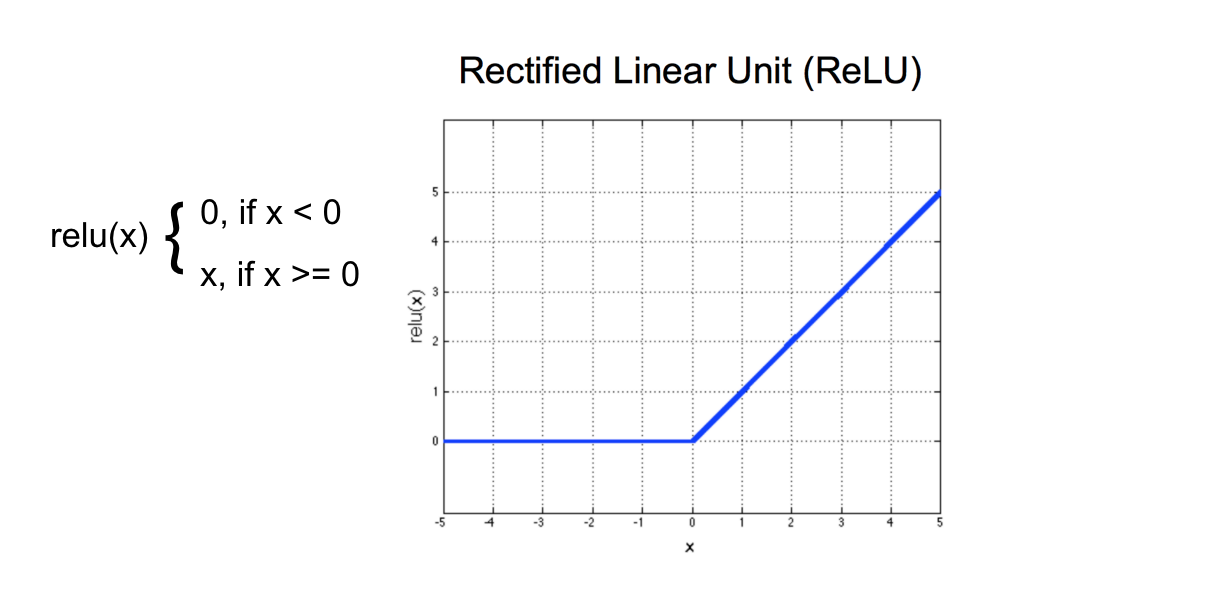
\includegraphics[scale=0.35]{figures/relu_ex.png}
            \caption{ReLU activation function in the}{positive interval is always 1.}\label{fig:relu_ex}
        \end{center}
    \end{figure}
\end{flushleft}
The AlexNet architecture introduced the use of ReLU (Rectified Linear Unit) Nonlinearity, which is a more efficient activation function than the previously used Tanh or sigmoid functions. It can be represented as: $f(x)=\max(0, x)$, where x is the input value. The paper shows that using ReLUs, AlexNet could achieve a 25\% training error rate six times faster than an equivalent network using $\tanh$. This was tested on the CIFAR-10 dataset\cite{Alexnet}. The function is applied after all the convolution and fully connected layers.

\subsubsection{Multi-GPU learning}
Multi-GPU learning is a method that allows for the parallelization of the training process across multiple GPUs. The authors utilized two GPUs to increase the network size, as the GPU at that time had a memory limit of 3GB\@. The network is split into two such as Figure\ref{fig:imagenet-6}, which communicated in specific layers to ensure they were not training two separate models. Therefore, the two-GPU net takes slightly less time to train than the one-GPU net.

\subsubsection{Dropout}
Dropout is a regularization technique that helps to prevent overfitting by randomly setting some neurons to zero during the training process. In AlexNet, dropout is applied to the first two fully-connected layers with a dropout rate of 0.5. This means that half of the neurons in these layers are ignored during each iteration of training. Dropout helps to improve the generalization performance of AlexNet on large-scale image recognition tasks.

\begin{flushleft}

    \begin{figure}[h!]
        \begin{center}
            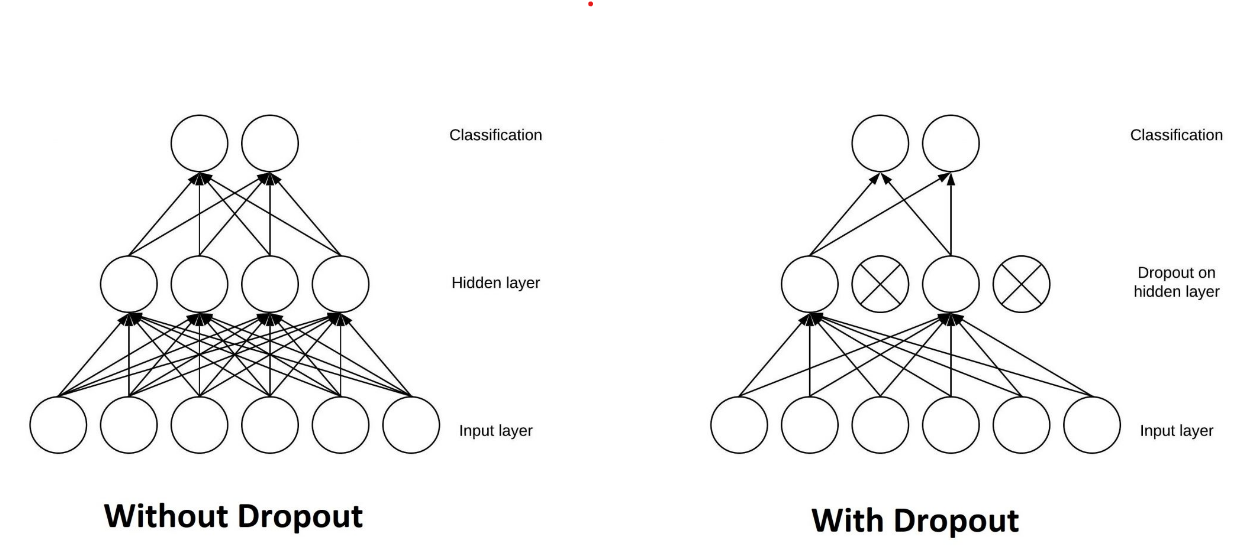
\includegraphics[scale=0.3]{figures/dropout.png}
            \caption{Dropout Neural Net Model\cite{baeldung_2020_how}.}\label{fig:dropout}
        \end{center}
    \end{figure}
\end{flushleft}

\subsection{VGGNet}
\subsubsection{The motivation behind the VGGNet Model}
The VGGNet model, officially known as the OxfordNet, was introduced in the paper titled
“Very Deep Convolutional Networks for Large-Scale Image Recognition”, presented at the
International Conference on Learning Representations (ICLR) in 2015. The VGGNet achieved
notable success in the ImageNet Large Scale Visual  Recognition Challenge (ILSVRC) in 2014,
showcasing the model’s mobility to excel in large-scale image classification tasks. In particular,
it achieved a test accuracy of 92.7 percent in ImageNet, a dataset containing more than 14 million
training images across 1000 object classes, paving the way for subsequent research in deep learning
and inspiring the exploration of even deeper neural network architectures.
\subsubsection{Architecture}
\paragraph{Deep Dark Fantasy} The general architecture of the VGGNet model is much deeper in comparison to that of AlexNet, which was a significant advancement at the time of its creation. One of its variants is VGG16 consists of 16 weight layers including 13 convolutional layers, and 3 fully-connected layers, with a total of 138 million parameters.\cite{tammina2019transfer} This depth is beneficial for its hierarchical feature learning. Deeper networks can learn robust and discriminative representations of features. Each layer in the network can capture increasingly abstract and complex features. This hierarchy allows the network to understand patterns at multiple levels of granularity. Another variant of VGGNet is VGG19, which has the similar structure of VGG16, except for the insertion of three more convolutional layers. In general, while maintaining the same structure and size of fully connected layers, VGG19 is deeper than VGG16 with 19 layers, potentially capturing more intricate features from images. Moreover, with more layers, VGG19 is computationally more intensive both in terms of memory and processing power compared to VGG16, but it does not indicate that there is a significant difference in the output of these models. The performance improvements gained by utilizing two VGGNet variants are marginal, especially in scenarios where training data might not be extensive enough to fully leverage the deeper architecture. Furthermore, the pre-trained VGG16 model can be fine-tuned for various tasks, which refers to the process of taking a pre-trained neural network and further training it on a new dataset or for a specific task, also known as transfer learning. In this case, the VGGNet models, including two variants VGG16 and VGG19, are already trained on ImageNet, which comprises over 14 million training images with thousands of disparate categories. Trained on huge datasets, the model has learned a good representation of low level features such as spatial, edges, rotation, lightning, shapes and these features can be shared across to enable the knowledge be leveraged and act as a feature extractor for new images in different computer vision problems based on the principles of transfer learning, even when the new images are of completely different categories from the source dataset.

\begin{figure}
    \begin{center}
        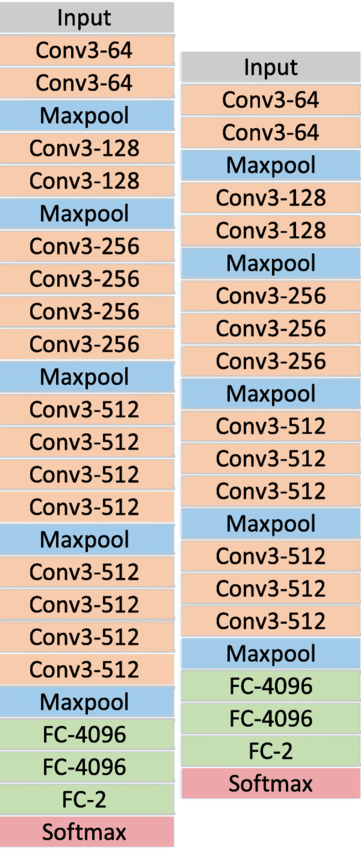
\includegraphics[width=0.4\textwidth]
        {figures/VGG_arc_compare.png}
        \caption{The architecture of VGG19 and VGG16.}\label{fig:picture}
    \end{center}
\end{figure}

\paragraph{Stacks of Smaller Convolutional Filters}
Rather than using relatively large receptive fields in the  first convolutional layers, multiple tiny $3\times3$ receptive
fields are selected throughout the whole net, which are convolved with the input at every pixel with a stride of 1.
The presented figures delineate that a stack of two $3\times3$ convolutional layers has an effective receptive field of $5\times5$.
Hence, it can be concluded that a stack of three $3\times3$ convolutional filters has an effective receptive field of $7\times7$.\\
Assuming it is obvious that stacks of small-kernel convolution layers have equal sized receptive fields, what makes them
a more optimal choice? The initial point is incorporating more rectification layers instead of s single one, on the grounds
that more non-linear activation layers accompany the convolutional layers, reducing the network’s tendency to over-fit during
training exercises, improving the decision functions and allowing the network to converge quickly. In addition, with a small
receptive field, a stack of $3\times3$ convolution filters have fewer parameters to train,\cite{VGG} saving computational
resources needed for training and inference, hence offering lower computational complexity.

\subsection{ResNet}
ResNet is an innovative result realized by a team of Microsoft researchers during participating the ILSVRC 2015, with the ultimate grand achievement is the first place of the competition by using multiple ensembles rooted from ResNet. Its original paper\cite{ResNet}, has gained substantial citations and is considered one of the most important contributions in the field of Computer Vision.

\subsubsection{Addressed problems}

\paragraph{Main problems} With the rapid development of convolutional neural networks after the success of VGGNet\cite{VGG}, various networks have been created based on the idea of VGG, “the deeper, the better”. Despite multiple slight differences in terms of layers or activation functions in those models, the same technique aiming at creating a model that was “deep enough” was utilized popularly at that time. However, a new problem was raised questioning the “deepness” of any CNN models: “How deep can a model be extended?”. The problem is called the degradation phenomenon, when a deeper version of a CNN model performs worse than its shallower counterparts. This experiment was shown in the paper of ResNet, when the authors trained 2 plain models and compared their performance, as shown in \ref{fig:ResNet_intro}. It is clear that the 20-layer model performed better than its deeper counterpart in both training and testing set. This graph also showed that the degradation phenomenon was not correlated with the overfitting problem \cite{overfitting_overview}, as the training error of the 56-layer model was higher than the 20-layer one and no divergence between the training error and the testing error was found. The authors argued that this phenomenon is caused when an already sufficiently deep model gets deeper, then its accuracy and training error would saturate earlier instead of achieving its efficient local extremum.

\begin{figure}
    \begin{center}
        \includegraphics[width=0.45\textwidth]{figures/ResNet_intro_compare.png}
        \caption{Training error (left) and test error (right) on CIFAR-10
            with 20-layer and 56-layer “plain” networks. The image was taken from the ResNet paper \cite{ResNet}.}\label{fig:ResNet_intro}
    \end{center}
\end{figure}

\paragraph{The pitfall of vanishing gradients} The degradation phenomenon mentioned above is currently still a controversial topic, when many sources \cite{visoai, Datagen_2023,GeeksforGeeks_2023} agree that this phenomenon is rooted from the vanishing gradients problem \cite{exp_vanishing_grad_1,exp_vanishing_grad_2}. This is indeed a valid reason since the gradients would gradually decay through each individual layer in the backpropagation phase. However, the authors of ResNet argued that the vanishing gradients problem has little effect on the model causing the degradation phenomenon. “We argue that this optimization difficulty is unlikely to be caused by vanishing gradients. These plain networks are trained with BN, which ensures forward propagated signals to have non-zero variances. We also verify that the backward propagated gradients exhibit healthy norms with BN. So neither forward nor backward signals vanish.”, stated by Kaiming He et al. in their paper \cite{ResNet}. Based on this argument, they argued that the degradation phenomenon was indeed a natural dilemma arising from the action of deepening any CNN models. This argument directly opposes the effect of the vanishing gradients problem on deep models, which would require that more proof and experiments must be conducted to approve any sides. However, despite the different reasoning of the degradation phenomenon, one of the same goals of any models created till now is avoiding this problem.

\subsubsection{Architecture}

\paragraph{Skip connections} Mathematically, defining a residual block with a skip connection as: \[y=\uppercase{\gamma}(x) + x\] With $\uppercase{\gamma}(x)$ represents a generalized convolutional mapping with an activation function. The equation strictly illustrates combining input \(x\) with \(\uppercase{\gamma}(x)\) through addition expression. A skip connection is a pathway for any input feature map to flow to the output of the next layer. The intuition behind this technique resembles the process of a person reviewing a picture one more time that has not seen for a long time. Adding the input to the output feature map is believed to make the model “remember” its input, since any processing or calculation that input went through may make the output completely unrelated. Moreover, many sources of information about ResNet besides the authors agree that these skip connections will alleviate the vanishing gradients problem, hence could help the model to have a greater amount of layers.

\begin{figure}
    \begin{center}
        \includegraphics[width=0.4\textwidth]{figures/ResNet_architecture.png}
        \caption{Architecture of ResNet compared to plain models. The image was taken from the ResNet paper \cite{ResNet}.}
        \label{fig:ResNet_architecture}
    \end{center}
\end{figure}

\paragraph{The general architecture} Since skip connections can be used as an identity mapping in any CNN models, the proposed ResNet would have many layers, from 34 to 151 layers preferably. The skip connections are utilized in each layer, as shown in \ref{fig:ResNet_architecture}. The proposed ResNet model resembles the VGGNet in terms of using small kernel size for convolutional layers and stacking a sufficient amount of these layers. The skip connections can be directly used when the input and output are of the same dimensions (solid line shortcuts in \ref{fig:ResNet_architecture}). When the dimensions increase (dotted line shortcuts in \ref{fig:ResNet_architecture}), there are 2 options: (A) The shortcut still performs identity mapping, with extra zero entries padded for increasing dimensions. This option introduces no extra parameter; (B) The projection shortcut is used to match dimensions (done by $1\times1$ convolutions). For both options, when the shortcuts go across feature maps of two sizes, they are performed with a stride of 2.

\subsubsection{Applications}

The invention of ResNet sparks the utilization of that same structure, especially the skip connections or residual blocks, in many CNN models not only in the Computer Vision field but also a greater, older field which is Natural Language Processing. Some impactful architectures developed based on ResNet are ResNeXt \cite{ResNeXt} and DenseNet \cite{DenseNet}, where residual blocks and skip connections are implemented differently to tackle the weaknesses of ResNet. In addition, those skip connections (or preferably called identity mapping), are utilized in Transformer \cite{Transformer}, which is an evolutionary architecture that outperformed any forms of CNN in NLP. The same architecture was also widely used to create different types of Transformer models in the Computer Vision field, such as ViT \cite{ViT} or Swin \cite{Swin}. The skip connections used in Transformer sequentially made the Attention blocks in this model a new type of residual blocks.

\subsection{YOLO}

\subsubsection{Initial YOLO model (YOLOv1)}
\paragraph{Initial problem} Prior to the initial model of YOLO, object detection was based on repurposing classifiers. According to the author of the first model in the YOLO family, they wanted a new approach to the task, framing object detection as a regression problem with “spatially separated bounding boxes and associated class probabilities” \cite{redmon2016look}.

\paragraph{Workflow} The model divides the input image into grid cells, each responsible for predicting several bounding boxes and their corresponding confidence score [1p]. The model then eliminates some bounding boxes around an object with a confidence score lower than a predefined threshold. If multiple bounding boxes are still left, then the model applies non-max suppression to select the one with the highest confidence score \cite{terven2023comprehensive, datacampYOLOObject}.

\paragraph{Architecture} The initial YOLO model consists of 24 convolutional layers, as in the table below, with leaky rectified linear unit activation (Leaky ReLU) functions except for the final layer using the linear activation function, followed by 2 fully-connected layers at the end. The output is the $7\times7\times30$ tensor of prediction \cite{redmon2016look, terven2023comprehensive}.

\begin{figure*}
    \begin{center}
        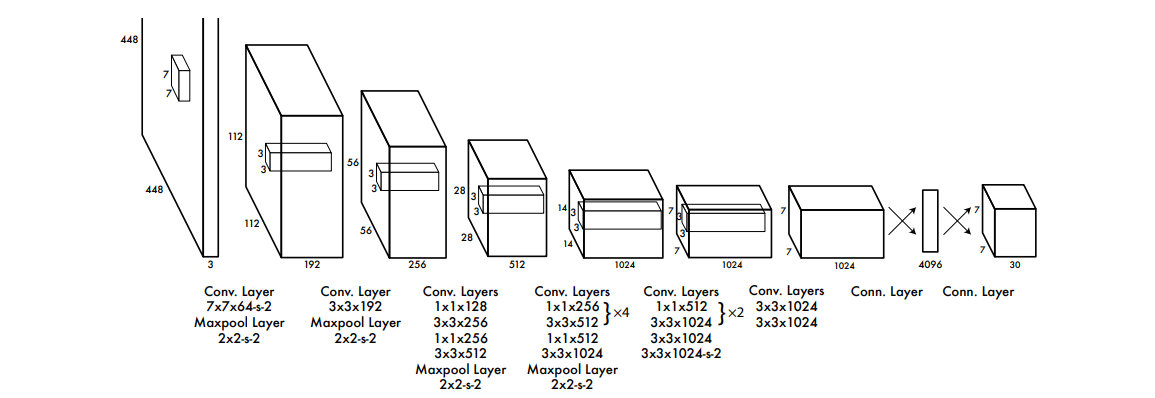
\includegraphics[width=0.8\textwidth]{figures/YOLO1.PNG}
        \caption{Architecture of YOLOv1.}
        \label{fig:picture1}
    \end{center}
\end{figure*}

\paragraph{Innovation} Their framing of the problem resulted in a single neural network as a complete pipeline performing object detection. This allows direct end-to-end optimization of the performance of the model. As a result, such a pipeline “straight from image pixels to bounding box coordinates and class probabilities” makes the model simple and, thus, faster than multi-part approaches such as R-CNN. Furthermore, this structure allows YOLO to observe the entire image, including the appearance of the classes as well as contextual information, to learn to generalize object representation and to perform with better accuracy \cite{redmon2016look}.

\paragraph{Limitations} Only a maximum of two boxes and one class can be predicted by a grid cell, meaning that the model has “strong spatial constraints on bounding box predictions”. This significantly reduces the ability of the model to predict small objects that appear in groups (such as a flock of birds), because the number of nearby objects that the model can predict is limited. Beyond that, the model “uses relatively coarse features for predicting bounding boxes” since those features have been downsampled  through its layers, thus making the model struggle in the generalization of objects in unfamiliar “aspect ratios or configurations”. Furthermore, the loss function treats the error in the small bounding box the same as in the large bounding box, though they differ in terms of the effect on the confidence score. This results in incorrect localization by the model \cite{redmon2016look}.

\paragraph{Legacy} Since the appearance of the initial model of YOLO (also known as YOLOv1), there have been many similar models taking the inspiration of YOLOv1 to improve its performance, eventually creating the family of YOLO models. YOLOv5 and YOLOv8, two variants of version 5 and version 8 of YOLO, are not exceptions. They are variants of the YOLO family, both developed by Glenn Jocher at Ultralytics \cite{githubGlennjocherOverview, ultralyticsHome}, both share the general architecture, inspired by YOLOv3, of three parts: the backbone, the head, and the neck. The backbone extracts the features and passes them to the neck, the neck combines those features into maps and passes them to the head, and the head performs its prediction job. They are also capable of different tasks than detection, such as classification and segmentation \cite{terven2023comprehensive, ultralyticsHome}.

\subsubsection{YOLOv5}

Months after YOLOv4 appeared, YOLOv5 was released by Glenn Jocher at Ultralytics \cite{terven2023comprehensive, githubGlennjocherOverview, ultralyticsHome}. It is similar to YOLOv4 but developed in PyTorch rather than Darknet (as both took inspiration from major innovations in YOLOv3) \cite{terven2023comprehensive}.

\paragraph{Changes compared to YOLOv1} The biggest change is the architecture. YOLOv5 uses the DarkNet53 backbone developed in YOLOv3, which has 53 convolution layers \cite{redmon2018yolov3}. The backbone consists of convolution modules (which is a convolution layer followed by Batch Normalization (BN) and SiLU activation) with CSP layers (which is the stacking of multiple convolution modules) and an SPPF layer at the end. The neck uses the CSP-PAN structure while the head uses that of YOLOv3 \cite{terven2023comprehensive}. The training strategy changes according to that of YOLOv4 \cite{bochkovskiy2020yolov4}. Version 5 of the YOLO family exercises multiple data augmentation techniques such as Mosaic \cite{bochkovskiy2020yolov4}, MixUp, HSV, etc. \cite{terven2023comprehensive, ultralyticsHome}, as well as hyperparameter evolution to automatically tune parameters for optimal performance \cite{ultralyticsHome}. The approach to prediction also changes. YOLOv5 adapts the anchor-box strategy from its predecessor of v3 \cite{terven2023comprehensive, redmon2018yolov3}, combined with its algorithm AutoAnchor to adjust the ill-fitted anchor-box \cite{terven2023comprehensive, ultralyticsHome}.

\begin{figure*}
    \begin{center}
        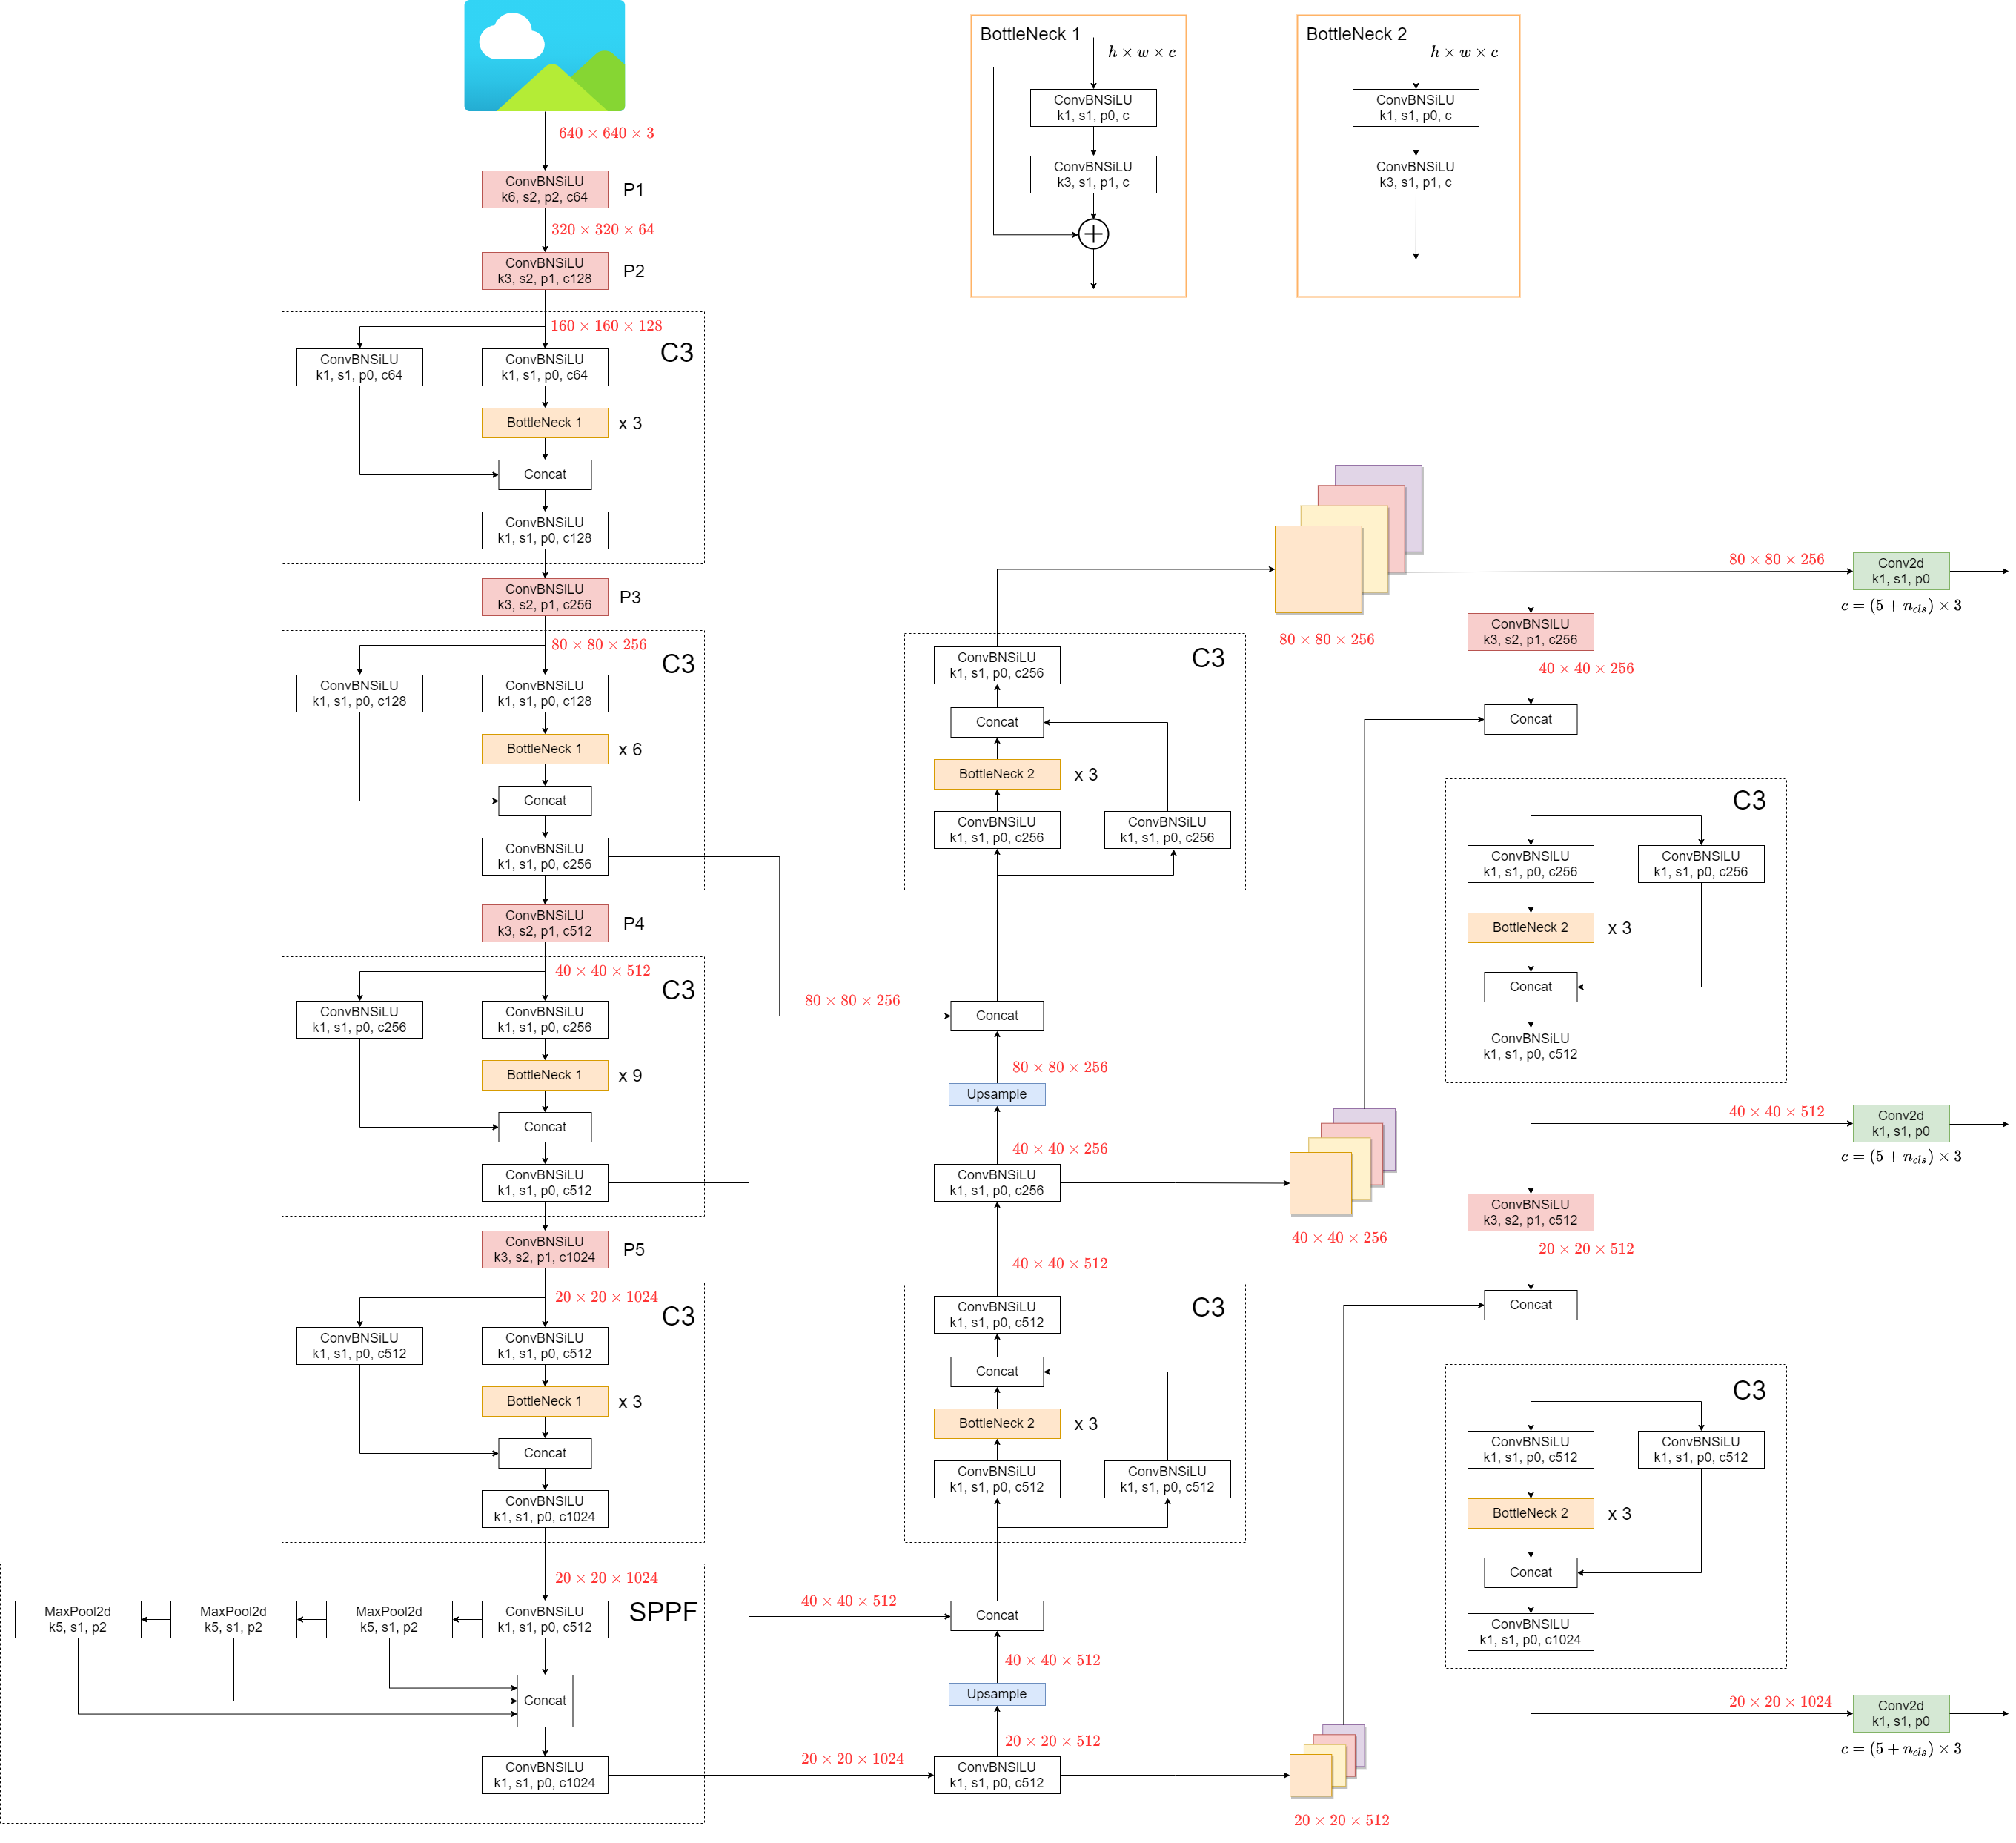
\includegraphics[width=0.8\textwidth]{figures/YOLO2.png}
        \caption{Architecture of YOLOv5.}
        \label{fig:picture2}
    \end{center}
\end{figure*}

\subsubsection{YOLOv8}

\paragraph{Similarities compared to YOLOv5} In January 2023, YOLOv8 was released as a directly improved version of YOLOv5 \cite{terven2023comprehensive, ultralyticsHome}. It uses a similar architecture to YOLOv5 except for the major change in the head.

\paragraph{Changes compared to YOLOv5} There is one major change in the architecture compared to YOLOv5, particularly in the head. YOLOv8 uses a decoupled head instead of a coupled one in YOLOv5. This allows the model to process each loss component independently, improving the model’s overall accuracy. Another notable change, but smaller, is the modified CSP layer, now called the C2f module \cite{terven2023comprehensive}. Another major change in the approach to prediction is the use of an anchor-free strategy. This reduces the computation complexity \cite{roboflowWhatYOLOv8} and compensates for the increasing number of parameters of the model \cite{githubGitHubUltralyticsultralytics}.

\begin{figure*}
    \begin{center}
        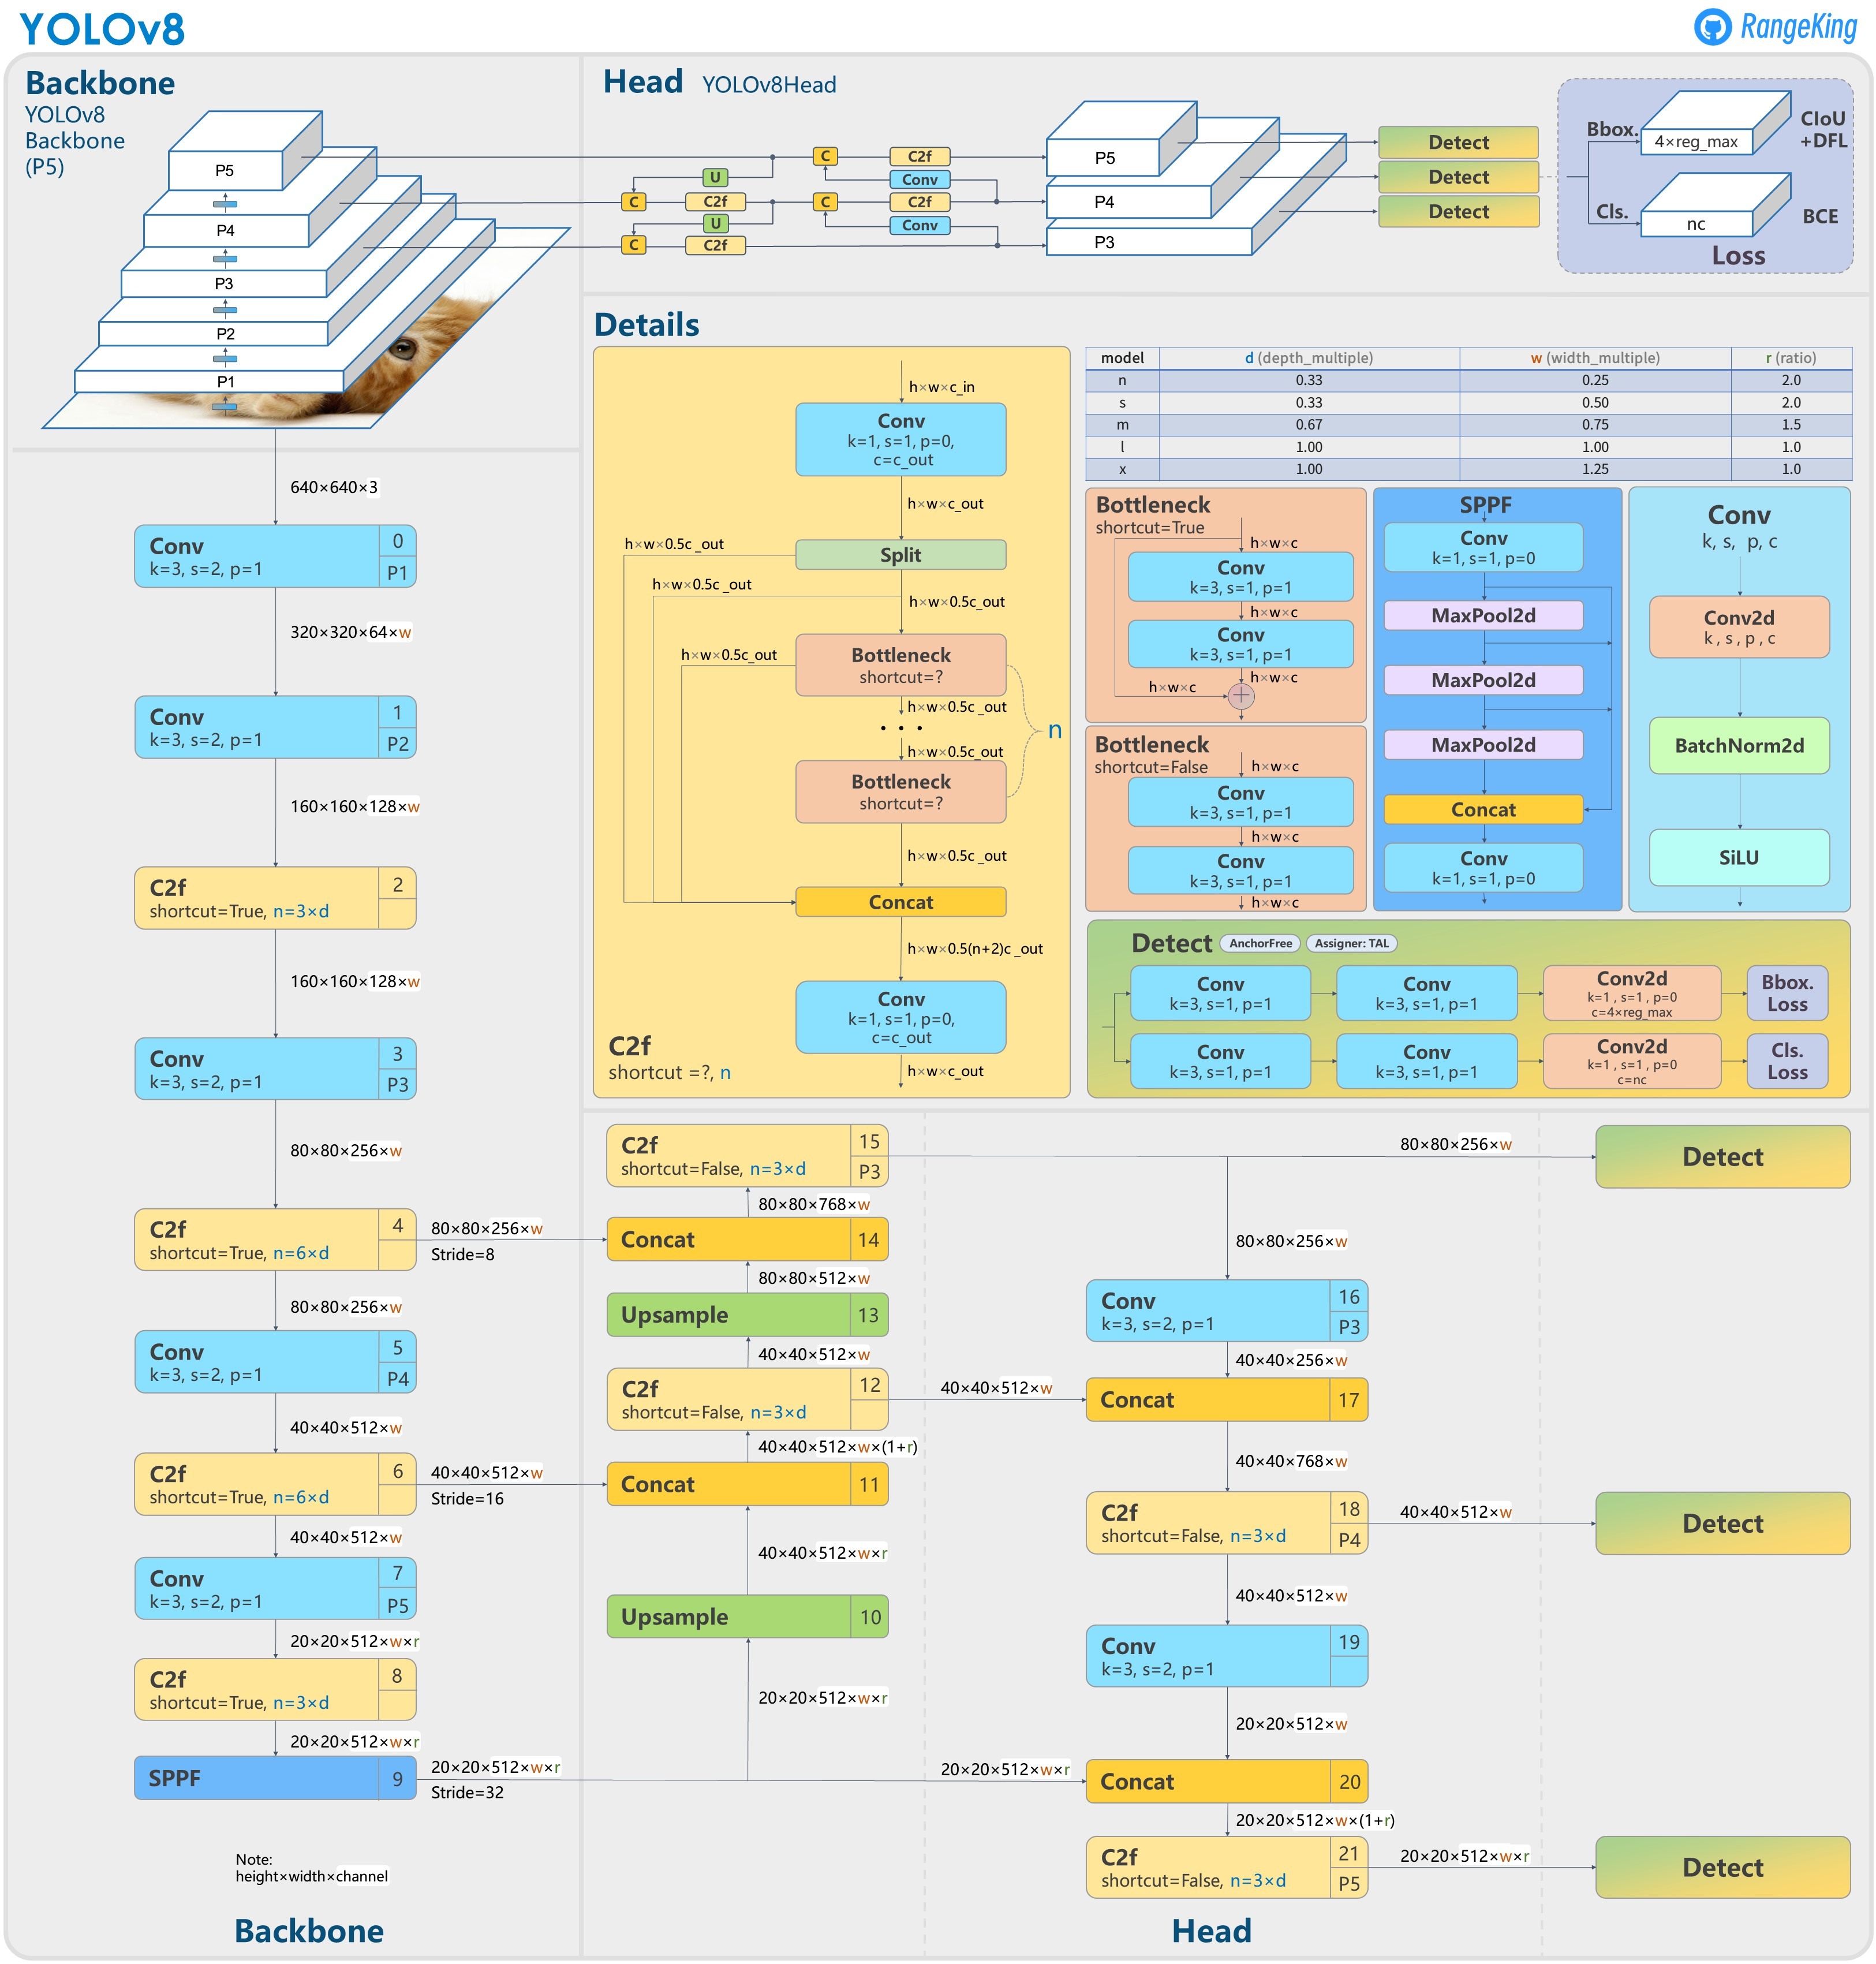
\includegraphics[width=0.8\textwidth]{figures/YOLO3.jpg}
        \caption{Architecture of YOLOv8.}
        \label{fig:picture3}
    \end{center}
\end{figure*}

%%%%%%%%% INSIGHTFUL COMPARISON

\section{Insightful summarization}

\begin{table}[h]
    \centering
    \label{tab:small_table}
    \scalebox{0.7}{\begin{tabular}{c|c c c c}
            \hline

            Models      & Release Date & Number of layers & Params (M) & Flops(G)\footnote{} \\
            \hline
            AlexNet     & 2012         & 8                & 61         & 0.715               \\
            VGGNet      & 2014         & 16 or 19         & 138-144    & 15.5-20             \\
            ResNet-50   & 2015         & 50               & 25.56      & 4.12                \\
            ResNet101   & 2015         & 101              & 44.55      & 7.85                \\
            Yolov5x-cis & 2020         & 19               & 48.1       & 15.9                \\
            Yolov8x-cls & 2023         & 53               & 57.4       & 154.8               \\
            \hline
        \end{tabular}}
    \caption{Data Comparision}
\end{table}
\footnotetext{GigaFlop (or Gflop) is a billion FLOPS. Here we take the data of the models that train with ImageNet dataset}

In addition to the aspects mentioned above, models that were created afterwards fixed the weaknesses of their predecessors. For instance,  AlexNet lacks explicit regularization techniques, making it prone to overfitting. VGGNet incorporates dropout, a regularization technique that randomly drops out a certain percentage of neurons during training. This forces the model to learn more robust and generalizable features, reducing overfitting and improving generalization performance. Although AlexNet implies dropout as well but only in the first two fully connected layers, VGGNet has it in both convolutional and connected layers. However, these two plain networks still confront the degradation problem when it comes to extending their architectures. Hence, ResNet was made to solve the vanishing gradients problem as the layers went deeper and deeper. Yolo is more like a pipeline that includes CNN models as backbone and others applies advanced techniques into training. Leading to a significant increase in FLOPs in terms of the numbers of params.

%%%%%%%%% CHALLENGES

\section{Challenges}
During the project, it is inevitable that we encounter multifaceted challenges, since AI research has never been effortless.
With regards to experience, almost all of the members had never approached the concept of machine learning in general and computer
vision in particular. It was necessary for us to read scientific papers, while each member had little opportunity and experience
to get used to reading journals. Hence, this procedure was so demanding, owing to the overwhelming number of journals of numerous
subjects; and at the same time, we lacked the orientation towards selecting appropriate articles for the required domain knowledge
in computer vision. Furthermore, this project involves interdisciplinary aspects where a lack of in-depth knowledge in certain domains
presented challenges, especially Linear Algebra. On the grounds that it plays a fundamental role in the field of Convolutional Neural
Networks, we were required to have a concrete foundation in some aspects of this discipline and apply them in computer vision tasks.
For instance, comprehending matrix operations demystifies the techniques and processes inside the convolutional and pooling layers;
or tensor representations simplify input handling, as when images are viewed as tensors, it is much easier to understand how CNNs
process data. In addition to this, a lack of resources serving for training purposes also hindered the project. Specifically, the
lack of powerful and reliable GPUs to train all chosen models and their variants necessitated more time. Ultimately, the project
operated under stringent time constraints due to the abundance of time spent on reading papers and acquiring sufficient knowledge
to build four selected AI models. The initial project schedule, carefully crafted to allow for comprehensive testing and logging
the results to compare the performance of them, was significantly compressed to meet the accelerated product launch timeline. However,
some procrastinations arose during the timeframe,  given that the time spent on researching was considerable and the time-consuming
process of training four models made the stage of logging and comparing metrics prolonged.

\section{Experiments}
\subsection{Dataset}
This study leverages the CIFAR-10 dataset for training and evaluation. CIFAR-10 consists of 60,000 $32\times32$ color images in 10 different classes, with 6,000 images per class. This dataset is widely used for image classification tasks, providing a diverse set of small-sized images for training robust models.

\subsection{Settings}
Typically, conducting a thorough experiment would be redundant since training and testing with each combination of hyperparameters would cost us a lot of time and resources. Therefore, we conducted an experiment which required a fixed setting and guaranteed homogeneity for all targeted models. The set of hyperparameters are configured in Tab \ref{tab:settings}.

\begin{table}
        \begin{center}
            \begin{tabular}{c|c}
                \hline
                \textbf{Settings} & \textbf{Value} \\
                \hline
                        Learning rate & 0.01\\
                        Epoch & 20 \\
                        Batch size & 64 - 128 \\
                        Input size & (224 x 224) \\
                        Augmentation & Random flip, RGB normalization \\
                        Dataset splits & Train-val-test (0.8-0.1-0.1) \\
                \hline
            \end{tabular}
            \caption{Settings for training and final comparison.}
            \label{tab:settings}
        \end{center}
\end{table}

It is not quite common to set the learning rate at $1e-2$ as it is considered unnecessary large, a more common learning rate is $1e-3$. However, for the sake of convergence speed of the chosen models, we chose this rate and adopted a “Reduce Learning Rate on Plateau” scheduler \cite{reduceonplateau} to have better results. Regarding the optimizer algorithm, Stochastic Gradient Descent \cite{SGD} was used because of its popularity and widely approved efficiency, with a weight decay of $0.01$ and $0.9$ momentum. Both training and testing procedures are conducted on a T4 GPU (with 15 GB VRam) provided by Google Colab and a local NVIDIA RTX 2060 (with 12 GB VRam).

\subsection{Result}
After 20 epochs of training, important metrics such as precision, recall and accuracy were logged\footnote[3]{YOLO metrics were not included. Please visit its official implemented pipeline at \url{https://github.com/ultralytics/ultralytics} for information of its metrics and training settings.}. Recorded values can be viewed in Fig \ref{fig:precision} and Fig \ref{fig:recall}.
\begin{figure}
        \begin{center}
            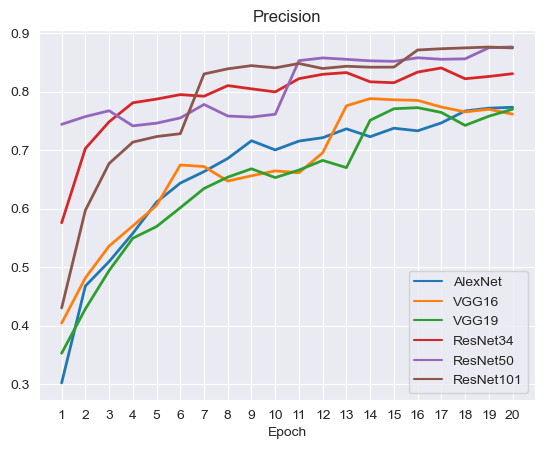
\includegraphics[width=0.45\textwidth]{figures/precision.png}
            \caption{Precision of all models on validation split. ResNet-50 and ResNet-101 both achieved the highest score.}
            \label{fig:precision}
        \end{center}
\end{figure}
\begin{figure}
        \begin{center}
            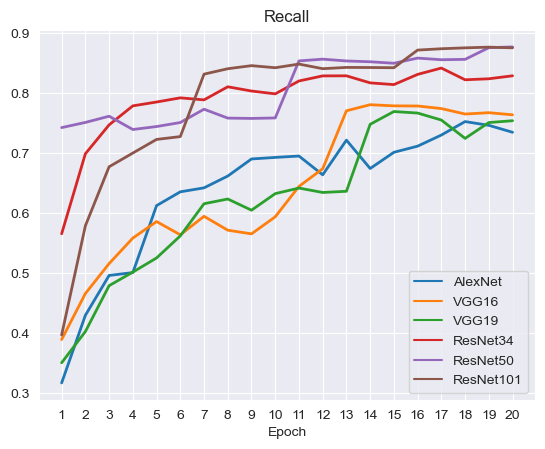
\includegraphics[width=0.45\textwidth]{figures/recall.png}
            \caption{Recall of all models on validation split. ResNet-50 and ResNet-101 both achieved the highest score.}
            \label{fig:recall}
        \end{center}
\end{figure}

The results of all tested models on the valuation set can be logically reasoned. These metrics indicate that a newer architecture would result in a better performance, since each model was proposed based on the fact that it has achieved or even surpassed the SOTA result at that time. AlexNet is the oldest model that has been proposed; hence, it performed generally worse compared to other models despite its unarguably good performance when compared to older Machine Learning techniques that mainly rely on feature extraction methods with mathematics. However, it is clear that these graphs reflect a quite opposite trend that we expected, which is the instability and fluctuation of the 2 VGG variants. At some points, including the $20^{th}$ epoch, both metrics of these 2 versions are lower than those of AlexNet. This strange phenomenon contradicts the common sense that we have introduced - the more parameters a model has, the more complex it is, the better it performs. Compared to AlexNet, VGGNet is far more complicated with a double amount of parameters that AlexNet has; which should imply that its variants would have better results. Regarding this peculiar problem, we propose a hypothesis for reasoning. We believe that each model has its own convergence timeline; which means that although both variants in this study perform worse than AlexNet, they should achieve better results when they are trained for longer time. Generally, 20 epochs are widely considered insufficient in order to evaluate the best result that a model can achieve; hence, training for sufficiently larger amount of epochs would result in a more logical output. 

Besides results logged after each epoch, an evaluation on the test set with $10,000$ images are also provided below.

\begin{table}[h]
        \centering
        \label{tab:small_table}
        \scalebox{1}{\begin{tabular}{c|c|c|c}
        \hline
        
        \textbf{Model} & \textbf{Accuracy} & \textbf{Precision} & \textbf{Recall} \\
        \hline
                AlexNet & 0.755 & 0.7726 & 0.755 \\
                VGG-16 & 0.7781 & 0.7773 & 0.7781 \\
                VGG-19 & 0.7739 & 0.7748 & 0.7739 \\
                ResNet-34 & 0.8431 & 0.8424 & 0.8431 \\
                ResNet-50 & 0.8653 & 0.8657 & 0.8653 \\
                ResNet101 & \underline{0.8848} & \underline{0.8851} & \underline{0.8848} \\
                Yolov8n-cls & \textbf{0.8896} & \textbf{0.8892} & \textbf{0.8896} \\
        \hline
        \end{tabular}}
        \caption{Result on test set. \textbf{Bold} values are largest, \underline{underline} values are second largest}
\end{table}

YOLOv8 nano with classification version achieved the best result, which is slightly better than the ResNet-101. YOLO is a complicated pipeline with different modules and parts that are regressed to produce the final result; hence its dominant result is understandable. In fact, considering only plain models would make ResNet stand out the most with its high performance in all of its 3 versions. This is also the reason why ResNet is widely utilized as a firm backbone for various pipelines and recent architectures.

\section{Teamwork}

\paragraph{Agile Scrum} is a dynamic, Agile-rooted project framework for complex product development, emphasizing collaboration, adaptability, and clear communication through roles like Product Owner, Scrum Master, and Development Team. Key ceremonies, such as Sprint Planning and Daily Scrum, ensure transparency and efficiency, making it widely recognized for delivering incremental value and enhancing project efficiency.

\subsection{Development cycle}

\paragraph{Week 1: Research and Project Scope Definition (22/10 - 28/10)} This week was pivotal as we delved into extensive research, culminating in the definition of our project scope and the formation of three specialized teams, each dedicated to a distinct AI model: YOLO, AlexNet, VGG, and ResNet.

\paragraph{Week 2: First Implementation and Model Training (29/10 - 4/11)} The second week marked the initiation of the implementation phase. This stage focused on the practical application of our research findings as we began the process of training each AI model—Yolo, AlexNet, VGG, and ResNet.

\paragraph{Week 3: Parameter Adjustment and Model Comparison (5/11 - 11/11)} In the third week, our focus shifted to fine-tuning the parameters of each AI model and conducting a comprehensive comparison. This crucial phase aimed to optimize the performance of YOLO, AlexNet, VGG, and ResNet while facilitating an insightful evaluation of their individual strengths and weaknesses.

\paragraph{Week 4: Presentation (12/11 - 18/11)} Entering the fourth week, our focus shifted to getting ready for the project presentation scheduled on 14/11/2023. This crucial week was all about putting together our findings, polishing our insights, and making sure our presentation on the convergence of CNNs and AI models was engaging and impactful.

\paragraph{Week 5: Reflection and Report (19/11 - 25/11)} In the last week of our 5-week Scrum journey, we turned our attention to creating the final report that captured everything we discovered about the convergence of CNNs and AI models. This week was crucial for summarizing our overall insights, lessons learned, and highlighting how our understanding evolved over the course of the journey.

\section{Conclusion}

Considering Real-World Applications and Scenarios:
When assessing the performance of YOLO, ResNet, VGGNet, and AlexNet in image classification, it's essential to examine their suitability for real-world scenarios. Each model comes with distinct strengths and weaknesses, shaping their applicability across different use cases. Understanding these attributes is crucial for deploying these models effectively in practical applications. Hence, this study delivered a comprehesive review of these models and provided an exhaustive comparison as a meaningful reference for individuals that are interested in this field.

% \subsection{Future Directions for Research} While YOLO stands out in image classification, there's room for ongoing research and improvement. Future endeavors could focus on optimizing the pipeline architecture for specific applications, enhancing adaptability to handle diverse object classes, and addressing identified limitations. Additionally, exploring ways to make YOLO more resource-efficient without compromising performance could broaden its deployment possibilities in resource-constrained environments.

\section{Acknowledgement}

We would like to express our deepest appreciation to all those who provided us the possibility to complete this report. A special gratitude we give to Dr. Le Trong Nhan, whose contribution in stimulating suggestions and encouragement, helped us to coordinate our project especially in writing this report.

    {\small
        \bibliographystyle{ieee}
        \bibliography{bibliography.bib}
    }

\end{document}